\newpage
\section{Несобственный интеграл}
\subsection{Определение несобственного интеграла}
\begin{definition}
    Если $f(x)\in \mathcal{R}[a,a_1],\ \forall a_1\in [a,b)$, то 
    \[\lim\limits_{a_1\to b-0}\int\limits_{a}^{a_1}f(x)\ dx=\int\limits_{a}^{b}f(x)\ dx\]
    называется несобственным интегралом первого рода.
    Если этот предел существует, то интеграл называется сходящимся, если не существует - расходящимся. 
\end{definition} 
\begin{definition}
    Если $f(x)\in \mathcal{R}[a,a_1],\ \forall a_1\in (a, +\infty)$, то
    \[\lim\limits_{a_1\to +\infty} \int\limits_{a}^{a_1}f(x)\ dx=\int\limits_{a}^{+\infty}f(x)\ dx\]
    называется несобственным интегралом второго рода. Если этот предел существует, то интеграл называется сходящимся, если не существует - расходящимся.
\end{definition} 
\begin{comm}
    В дальнейшем будем обозначать несобственные интегралы
    \[\int\limits_{a}^{\omega}f(x)\ dx\]
    где $\omega$ - число или знак\ $+\infty\ (-\infty)$.
\end{comm} 
\begin{comm}
    Если на отрезке интегрирования несобственного интеграла есть несколько особых точек, то интеграл сходится, если он сходится во всех своих особых точках. Такие интегралы также могут рассматриваться в дальнейших рассуждениях.
\end{comm}
\subsection{Критерий Коши сходимости несобственного интеграла}
\begin{theorem}
    Несобственный интеграл
    \[\int\limits_{a}^{\omega}f(x)\ dx\]
    сходится тогда и только тогда, когда
    \[\forall \epsilon>0\ \exists\ \delta\in [a,\omega),\ \forall x_1,x_2\in [\delta, \omega):\ \left|\ \int\limits_{x_1}^{x_2}f(t)\ dt\ \right|<\epsilon\]
\end{theorem} 
\begin{proof}
    Рассмотрим функцию
    \[F(x)=\int\limits_{a}^{x}f(t)\ dt\]
    и запишем критерий Коши существования предела $f(x)$ при $x \to \omega$.
    \[\forall \epsilon>0\ \exists\ \delta>0\ \forall x_1, x_2\in [\delta, \omega): |F(x_2)-F(x_1)|<\epsilon\]
    значит
    \[\left|\ \int\limits_{x_1}^{x_2}f(t)\ dt\ \right|=\left|\ \int\limits_{a}^{x_2}f(t)\ dt-\int\limits_{a}^{x_1}f(t)\ dt\ \right|=|F(x_2)-F(x_1)|<\epsilon\]
\end{proof} 
\subsection{Свойства несобственного интеграла}
\setcounter{thmcount}{0}
\begin{numtheorem}
    (Линейность)\\
    $\forall \alpha,\ \beta\in \R$ если существуют интегралы
    \[\int\limits_{a}^{\omega}f(x)\ dx,\ \int\limits_{a}^{\omega}g(x)\ dx\]
    то существует интеграл
    \[\int\limits_{a}^{\omega}(\alpha f(x)+\beta g(x))=\alpha\cdot \int\limits_{a}^{\omega}f(x)\ dx+\beta\cdot \int\limits_{a}^{\omega}g(x)\ dx\]
\end{numtheorem}
\begin{numtheorem}
    (Интегрирование по частям)\\
    Пусть $f(x),\ g(x)\in \mathcal{C}^1[a,\omega)$. Если существуют два объекта из трех:
    \[\int\limits_{a}^{\omega} f(x)g'(x)\ dx,\ \int\limits_{a}^{\omega}f'(x)g(x)\ dx,\ \lim\limits_{x\to \omega}f(x)g(x)\]
    то существует и третий и верна формула
    \[\int\limits_{a}^{\omega}f(x)g'(x)\ dx=f(x)g(x)|_a^{\omega}-\int\limits_{a}^{\omega}f'(x)g(x)\ dx\]
\end{numtheorem}  
\begin{numtheorem}
    (Замена переменной)\\
    Рассмотрим несобственный интеграл 
    \[\int\limits_{a}^{\omega}f(x)\ dx\]
    и пусть $\phi(t)\in \mathcal{C}^1[\alpha,\beta),\ a\leq \phi(t)\leq \omega,\ \phi(\alpha)=a,\ \lim\limits_{t\to \beta}\phi(t)=\omega$
    \[\int\limits_{a}^{\omega}f(x)\ dx=\int\limits_{\alpha}^{\beta} f(\phi(t))\phi'(t)\ dt\]
\end{numtheorem} 
\begin{numtheorem}
    Пусть существуют несобственные интегралы
    \[\int\limits_{a}^{\omega}f(x)\ dx,\ \int\limits_{a}^{\omega}g(x)\ dx\]
    Если $f(x)\leq g(x)$, то
    \[\int\limits_{a}^{\omega}f(x)\ dx\leq \int\limits_{a}^{\omega}g(x)\ dx\]
\end{numtheorem} 
\begin{numtheorem}
    Если $\forall a'\in [a, \omega)$ существует интеграл
    \[\int\limits_{a}^{a'}f(x)\ dx\]
    а также существует несобственный интеграл
    \[\int\limits_{a}^{\omega}|f(x)|\ dx\]
    то
    \[\left|\int\limits_{a}^{\omega}f(x)\ dx\right|\leq \int\limits_{a}^{\omega}|f(x)|\ dx\]
\end{numtheorem} 
\begin{definition}
    Если существует интеграл
    \[\int\limits_{a}^{\omega}|f(x)|\ dx\]
    то интеграл
    \[\int\limits_{a}^{\omega}f(x)\ dx\]\
    называется абсолютно сходящимся.
\end{definition} 
\begin{statement}
    Если $\forall a'\in [a, \omega)$ существует интеграл
    \[\int\limits_{a}^{a'}f(x)\ dx\]
    и интеграл
    \[\int\limits_{a}^{\omega}|f(x)|\ dx\]
    сходится, то интеграл
    \[\int\limits_{a}^{\omega}f(x)\ dx\]
    сходится
\end{statement} 
\begin{proof}
    По критерию Коши и неравентсву
    \[\left|\int\limits_{a_1}^{a_2}f(x)\ dx\right|\leq \int\limits_{a_1}^{a_2}|f(x)|\ dx<\epsilon\]
\end{proof} 
\begin{definition}
    Сходяшийся интеграл 
    \[\int\limits_{a}^{\omega}f(x)\ dx\]
    называется условно сходящимся, если интеграл 
    \[\int\limits_{a}^{\omega}|f(x)|\ dx\]
    расходится.
\end{definition} 
\begin{example} Рассмотрим функцию $f(x)$, которая задается последовательностью треугольников, у которых основание лежит на оси абсцисс, причем центрами оснований являются точки $1,2,3,\dots$, вершиной k-го треугольника является точка $(k,k)$, а также площади треугольников составляют бесконечно убывающую геометрическую прогрессию $\frac{1}{2}, \frac{1}{4}, \frac{1}{8}, \dots$. Построенная функция неограничена на $[0,+\infty)$, но интерал от нее сходится.
    \[\int\limits_{0}^{+\infty}f(x)\ dx=\sum\limits_{i=1}^{\infty}\frac{1}{2^i}=1\] 
    \newpage
    \[
    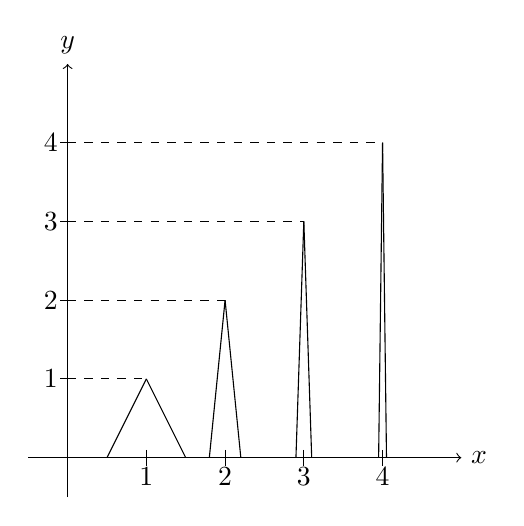
\begin{tikzpicture}[scale=1]
        \draw[->] (-0.5, 0) -- (5, 0) node[right] {$x$};
        \draw[->] (0, -0.5) -- (0, 5) node[above] {$y$};
    
        \foreach \x in {1, 2, 3, 4} {
            \draw (\x, 0) node[below] {\x};
            \draw (\x, 0.1) -- (\x, -0.1);
        }
    
        \foreach \y in {1, 2, 3, 4} {
            \draw (0, \y) node[left] {\y};
            \draw (0.1, \y) -- (-0.1, \y);
        }

        \draw[-] (0.5, 0) -- (1, 1);
        \draw[-] (1, 1) -- (1.5, 0);

        \draw[-] (1.8, 0) -- (2, 2);
        \draw[-] (2, 2) -- (2.2, 0);

        \draw[-] (2.9, 0) -- (3, 3);
        \draw[-] (3, 3) -- (3.1, 0);

        \draw[-] (3.95, 0) -- (4, 4);
        \draw[-] (4, 4) -- (4.05, 0);

        \draw[dashed] (0, 1) -- (1, 1);
        \draw[dashed] (0, 2) -- (2, 2);
        \draw[dashed] (0, 3) -- (3, 3);
        \draw[dashed] (0, 4) -- (4, 4);
    \end{tikzpicture}
\]
\end{example}
\subsection{Признаки сходимости несобственных интегралов}
\begin{theorem}
    (Признак Вейерштрасса)\\
    Пусть $0\leq f(x)\leq g(x)$ на $[a,\omega)$
    \begin{enumerate} 
    \item Если существует интеграл
    \[\int\limits_{a}^{\omega}g(x)\ dx\]
    то существует интеграл
    \[\int\limits_{a}^{\omega}f(x)\ dx\]
    \item Если не существует интеграла
    \[\int\limits_{a}^{\omega}f(x)\ dx\]
    то не существует интеграла
    \[\int\limits_{a}^{\omega}g(x)\ dx\]
\end{enumerate}
\end{theorem} 
\begin{proof}
    Рассмотрим функции 
    \[F(x)=\int\limits_{a}^{x}f(t)\ dt,\ G(x)=\int\limits_{a}^{x}g(t)\ dt\]
    заметим, что они неубывающие, а также
    \[f(x)\leq g(x) \Rightarrow F(x)\leq G(x)\]
    \begin{enumerate}
        \item Пусть $G(x)\to C \Rightarrow F(x)\leq C \Rightarrow$ по теореме Вейерштрасса существует предел $F(x)$.
        \item Поскольку $F(x)$ неубывает и у нее не существует предела, то $F(x)\to +\infty$, но так как $F(x)\leq G(x)$, то и $G(x)\to +\infty$.
    \end{enumerate}
\end{proof}
\begin{theorem}
    Пусть $0\leq f(x)\leq g(x)$ и существует предел
    \[\lim\limits_{x\to \omega}\frac{f(x)}{g(x)}=1\]
    Тогда интегралы
    \[\int\limits_{a}^{\omega}f(x)\ dx,\ \int\limits_{a}^{\omega}g(x)\ dx\] 
    сходятся или расходятся одновременно.
\end{theorem} 
\begin{proof}
    $\forall \epsilon>0\ \exists\ A,\ \forall x\in [A, \omega)$:
    \[\left|\frac{f(x)}{g(x)}-1\right|<\epsilon \Rightarrow 1-\epsilon<\frac{f(x)}{g(x)}<1+\epsilon\]
    значит
    \[(1-\epsilon)\cdot g(x)<f(x)<(1+\epsilon)\cdot g(x)\]
    далее воспользуемся признаком Вейерштрасса.
\end{proof} 
\begin{theorem}
    (Признаки Абеля и Дирихле)\\
    Пусть $f(x)\in \mathcal{C}[a,\omega),\ g(x)$ монотонна на $[a,\omega)$, а также $|f(x)|\leq C,\ |g(x)|\leq C$. Тогда 
    \begin{itemize}
        \item[($\mathcal{A}$):] Если существует интеграл 
        \[\int\limits_{a}^{\omega}f(x)\ dx\]
        то существует интеграл
        \[\int\limits_{a}^{\omega}f(x)g(x)\ dx\]
        \item[($\mathcal{D}$):] Если $g(x)\to 0$ при $x\to \omega$ и
        \[\left|\int\limits_{a}^{a'}f(x)\ dx\right|\leq C,\ \forall a'\in [a,\omega)\]
        то существует интеграл
        \[\int\limits_{a}^{\omega}f(x)g(x)\ dx\]
    \end{itemize}
\end{theorem} 
\begin{proof}
    \begin{multline*}
        \left|\int\limits_{x_1}^{x_2}f(x)g(x)\ dx\right|=\left|g(x_1)\cdot \int\limits_{x_1}^{c}f(x)\ dx+g(x_2)\cdot \int\limits_{c}^{x_2}f(x)\ dx\right|\leq\\\
        \leq |g(x_1)|\cdot \left|\int\limits_{x_1}^{c}f(x)\ dx\right|+|g(x_2)|\cdot \left|\int\limits_{c}^{x_2}f(x)\ dx\right|\leq
    \end{multline*} 
    $(\mathcal{A}):\ \leq C\cdot 2\epsilon$\\
    $(\mathcal{D}):\ \leq \epsilon \cdot 4C$
\end{proof} 
\begin{example} Интеграл 
    \[\int\limits_{1}^{+\infty}\frac{\sin{x}}{x}\ dx\]
    сходится, но интеграл
    \[\int\limits_{1}^{+\infty}\left|\frac{\sin{x}}{x}\right|\ dx\]
    расходится, так как
    \[\frac{1}{2x}-\frac{\cos{2x}}{2x}=\frac{1-\cos{2x}}{2x}=\frac{\sin^2{x}}{x}\leq \frac{|\sin{x}|}{x}\]
\end{example}
\subsection{Главное значение интеграла в смысле Коши}
\begin{definition}
    Пусть $f(x)$ определена на $\R$ и $f(x)\in \mathcal{R}[a,b],\ \forall a,b$. Величина
    \[\lim\limits_{A\to +\infty}\int\limits_{-A}^{A}f(x)\ dx=\text{v.p.} \int\limits_{-\infty}^{+\infty}f(x)\ dx\]
    называется главным значением интеграла в смысле Коши. % Интегралом несобств не является
\end{definition} 
\begin{comm}
    Главное значение интеграла в смысле Коши не является несобственным интегралом.
\end{comm} 
\begin{theorem}
    Главное значение интеграла в смысле Коши существует, если сходится несобственный интеграл
    \[\int\limits_{0}^{+\infty}(f(x)+f(-x))\ dx\]
\end{theorem} 
\begin{proof}
    \[f(x)=\frac{f(x)+f(-x)}{2}+\frac{f(x)-f(-x)}{2}\]
    Возьмем интеграл от $-A$ до $A$, второе слагаемое всегда ноль.
\end{proof} 
\begin{comm}
    Аналогично определяется главное значение с особенностью в точке $c\in (a,b)$:
    \[\text{v.p.}\int\limits_{a}^{b}f(x)\ dx=\lim\limits_{\epsilon\to 0+0}\left(\int\limits_{a}^{c-\epsilon}f(x)\ dx+\int\limits_{c+\epsilon}^{b}f(x)\ dx\right)\]
\end{comm} 